
%% bare_conf.tex
%% V1.4b
%% 2015/08/26
%% by Michael Shell
%% See:
%% http://www.michaelshell.org/
%% for current contact information.
%%
%% This is a skeleton file demonstrating the use of IEEEtran.cls
%% (requires IEEEtran.cls version 1.8b or later) with an IEEE
%% conference paper.
%%
%% Support sites:
%% http://www.michaelshell.org/tex/ieeetran/
%% http://www.ctan.org/pkg/ieeetran
%% and
%% http://www.ieee.org/

%%*************************************************************************
%% Legal Notice:
%% This code is offered as-is without any warranty either expressed or
%% implied; without even the implied warranty of MERCHANTABILITY or
%% FITNESS FOR A PARTICULAR PURPOSE! 
%% User assumes all risk.
%% In no event shall the IEEE or any contributor to this code be liable for
%% any damages or losses, including, but not limited to, incidental,
%% consequential, or any other damages, resulting from the use or misuse
%% of any information contained here.
%%
%% All comments are the opinions of their respective authors and are not
%% necessarily endorsed by the IEEE.
%%
%% This work is distributed under the LaTeX Project Public License (LPPL)
%% ( http://www.latex-project.org/ ) version 1.3, and may be freely used,
%% distributed and modified. A copy of the LPPL, version 1.3, is included
%% in the base LaTeX documentation of all distributions of LaTeX released
%% 2003/12/01 or later.
%% Retain all contribution notices and credits.
%% ** Modified files should be clearly indicated as such, including  **
%% ** renaming them and changing author support contact information. **
%%*************************************************************************


% *** Authors should verify (and, if needed, correct) their LaTeX system  ***
% *** with the testflow diagnostic prior to trusting their LaTeX platform ***
% *** with production work. The IEEE's font choices and paper sizes can   ***
% *** trigger bugs that do not appear when using other class files.       ***                          ***
% The testflow support page is at:
% http://www.michaelshell.org/tex/testflow/



\documentclass[conference]{IEEEtran}
% Some Computer Society conferences also require the compsoc mode option,
% but others use the standard conference format.
%
% If IEEEtran.cls has not been installed into the LaTeX system files,
% manually specify the path to it like:
% \documentclass[conference]{../sty/IEEEtran}


%\usepackage[]{algorithm2e}


% Some very useful LaTeX packages include:
% (uncomment the ones you want to load)


% *** MISC UTILITY PACKAGES ***
%
%\usepackage{ifpdf}
% Heiko Oberdiek's ifpdf.sty is very useful if you need conditional
% compilation based on whether the output is pdf or dvi.
% usage:
% \ifpdf
%   % pdf code
% \else
%   % dvi code
% \fi
% The latest version of ifpdf.sty can be obtained from:
% http://www.ctan.org/pkg/ifpdf
% Also, note that IEEEtran.cls V1.7 and later provides a builtin
% \ifCLASSINFOpdf conditional that works the same way.
% When switching from latex to pdflatex and vice-versa, the compiler may
% have to be run twice to clear warning/error messages.






% *** CITATION PACKAGES ***
%
%\usepackage{cite}
% cite.sty was written by Donald Arseneau
% V1.6 and later of IEEEtran pre-defines the format of the cite.sty package
% \cite{} output to follow that of the IEEE. Loading the cite package will
% result in citation numbers being automatically sorted and properly
% "compressed/ranged". e.g., [1], [9], [2], [7], [5], [6] without using
% cite.sty will become [1], [2], [5]--[7], [9] using cite.sty. cite.sty's
% \cite will automatically add leading space, if needed. Use cite.sty's
% noadjust option (cite.sty V3.8 and later) if you want to turn this off
% such as if a citation ever needs to be enclosed in parenthesis.
% cite.sty is already installed on most LaTeX systems. Be sure and use
% version 5.0 (2009-03-20) and later if using hyperref.sty.
% The latest version can be obtained at:
% http://www.ctan.org/pkg/cite
% The documentation is contained in the cite.sty file itself.






% *** GRAPHICS RELATED PACKAGES ***
%
\ifCLASSINFOpdf
  % \usepackage[pdftex]{graphicx}
  % declare the path(s) where your graphic files are
  % \graphicspath{{../pdf/}{../jpeg/}}
  % and their extensions so you won't have to specify these with
  % every instance of \includegraphics
  % \DeclareGraphicsExtensions{.pdf,.jpeg,.png}
\else
  % or other class option (dvipsone, dvipdf, if not using dvips). graphicx
  % will default to the driver specified in the system graphics.cfg if no
  % driver is specified.
  % \usepackage[dvips]{graphicx}
  % declare the path(s) where your graphic files are
  % \graphicspath{{../eps/}}
  % and their extensions so you won't have to specify these with
  % every instance of \includegraphics
  % \DeclareGraphicsExtensions{.eps}
\fi
% graphicx was written by David Carlisle and Sebastian Rahtz. It is
% required if you want graphics, photos, etc. graphicx.sty is already
% installed on most LaTeX systems. The latest version and documentation
% can be obtained at: 
% http://www.ctan.org/pkg/graphicx
% Another good source of documentation is "Using Imported Graphics in
% LaTeX2e" by Keith Reckdahl which can be found at:
% http://www.ctan.org/pkg/epslatex
%
% latex, and pdflatex in dvi mode, support graphics in encapsulated
% postscript (.eps) format. pdflatex in pdf mode supports graphics
% in .pdf, .jpeg, .png and .mps (metapost) formats. Users should ensure
% that all non-photo figures use a vector format (.eps, .pdf, .mps) and
% not a bitmapped formats (.jpeg, .png). The IEEE frowns on bitmapped formats
% which can result in "jaggedy"/blurry rendering of lines and letters as
% well as large increases in file sizes.
%
% You can find documentation about the pdfTeX application at:
% http://www.tug.org/applications/pdftex





% *** MATH PACKAGES ***
%
%\usepackage{amsmath}
% A popular package from the American Mathematical Society that provides
% many useful and powerful commands for dealing with mathematics.
%
% Note that the amsmath package sets \interdisplaylinepenalty to 10000
% thus preventing page breaks from occurring within multiline equations. Use:
%\interdisplaylinepenalty=2500
% after loading amsmath to restore such page breaks as IEEEtran.cls normally
% does. amsmath.sty is already installed on most LaTeX systems. The latest
% version and documentation can be obtained at:
% http://www.ctan.org/pkg/amsmath





% *** SPECIALIZED LIST PACKAGES ***
%
%\usepackage{algorithmic}
% algorithmic.sty was written by Peter Williams and Rogerio Brito.
% This package provides an algorithmic environment fo describing algorithms.
% You can use the algorithmic environment in-text or within a figure
% environment to provide for a floating algorithm. Do NOT use the algorithm
% floating environment provided by algorithm.sty (by the same authors) or
% algorithm2e.sty (by Christophe Fiorio) as the IEEE does not use dedicated
% algorithm float types and packages that provide these will not provide
% correct IEEE style captions. The latest version and documentation of
% algorithmic.sty can be obtained at:
% http://www.ctan.org/pkg/algorithms
% Also of interest may be the (relatively newer and more customizable)
% algorithmicx.sty package by Szasz Janos:
% http://www.ctan.org/pkg/algorithmicx




% *** ALIGNMENT PACKAGES ***
%
%\usepackage{array}
% Frank Mittelbach's and David Carlisle's array.sty patches and improves
% the standard LaTeX2e array and tabular environments to provide better
% appearance and additional user controls. As the default LaTeX2e table
% generation code is lacking to the point of almost being broken with
% respect to the quality of the end results, all users are strongly
% advised to use an enhanced (at the very least that provided by array.sty)
% set of table tools. array.sty is already installed on most systems. The
% latest version and documentation can be obtained at:
% http://www.ctan.org/pkg/array


% IEEEtran contains the IEEEeqnarray family of commands that can be used to
% generate multiline equations as well as matrices, tables, etc., of high
% quality.




% *** SUBFIGURE PACKAGES ***
%\ifCLASSOPTIONcompsoc
%  \usepackage[caption=false,font=normalsize,labelfont=sf,textfont=sf]{subfig}
%\else
%  \usepackage[caption=false,font=footnotesize]{subfig}
%\fi
% subfig.sty, written by Steven Douglas Cochran, is the modern replacement
% for subfigure.sty, the latter of which is no longer maintained and is
% incompatible with some LaTeX packages including fixltx2e. However,
% subfig.sty requires and automatically loads Axel Sommerfeldt's caption.sty
% which will override IEEEtran.cls' handling of captions and this will result
% in non-IEEE style figure/table captions. To prevent this problem, be sure
% and invoke subfig.sty's "caption=false" package option (available since
% subfig.sty version 1.3, 2005/06/28) as this is will preserve IEEEtran.cls
% handling of captions.
% Note that the Computer Society format requires a larger sans serif font
% than the serif footnote size font used in traditional IEEE formatting
% and thus the need to invoke different subfig.sty package options depending
% on whether compsoc mode has been enabled.
%
% The latest version and documentation of subfig.sty can be obtained at:
% http://www.ctan.org/pkg/subfig




% *** FLOAT PACKAGES ***
%
%\usepackage{fixltx2e}
% fixltx2e, the successor to the earlier fix2col.sty, was written by
% Frank Mittelbach and David Carlisle. This package corrects a few problems
% in the LaTeX2e kernel, the most notable of which is that in current
% LaTeX2e releases, the ordering of single and double column floats is not
% guaranteed to be preserved. Thus, an unpatched LaTeX2e can allow a
% single column figure to be placed prior to an earlier double column
% figure.
% Be aware that LaTeX2e kernels dated 2015 and later have fixltx2e.sty's
% corrections already built into the system in which case a warning will
% be issued if an attempt is made to load fixltx2e.sty as it is no longer
% needed.
% The latest version and documentation can be found at:
% http://www.ctan.org/pkg/fixltx2e


%\usepackage{stfloats}
% stfloats.sty was written by Sigitas Tolusis. This package gives LaTeX2e
% the ability to do double column floats at the bottom of the page as well
% as the top. (e.g., "\begin{figure*}[!b]" is not normally possible in
% LaTeX2e). It also provides a command:
%\fnbelowfloat
% to enable the placement of footnotes below bottom floats (the standard
% LaTeX2e kernel puts them above bottom floats). This is an invasive package
% which rewrites many portions of the LaTeX2e float routines. It may not work
% with other packages that modify the LaTeX2e float routines. The latest
% version and documentation can be obtained at:
% http://www.ctan.org/pkg/stfloats
% Do not use the stfloats baselinefloat ability as the IEEE does not allow
% \baselineskip to stretch. Authors submitting work to the IEEE should note
% that the IEEE rarely uses double column equations and that authors should try
% to avoid such use. Do not be tempted to use the cuted.sty or midfloat.sty
% packages (also by Sigitas Tolusis) as the IEEE does not format its papers in
% such ways.
% Do not attempt to use stfloats with fixltx2e as they are incompatible.
% Instead, use Morten Hogholm'a dblfloatfix which combines the features
% of both fixltx2e and stfloats:
%
% \usepackage{dblfloatfix}
% The latest version can be found at:
% http://www.ctan.org/pkg/dblfloatfix




% *** PDF, URL AND HYPERLINK PACKAGES ***
%
%\usepackage{url}
% url.sty was written by Donald Arseneau. It provides better support for
% handling and breaking URLs. url.sty is already installed on most LaTeX
% systems. The latest version and documentation can be obtained at:
% http://www.ctan.org/pkg/url
% Basically, \url{my_url_here}.


\usepackage{listings}
\usepackage{amsmath}
\usepackage{graphicx}
\usepackage{hyperref}

% *** Do not adjust lengths that control margins, column widths, etc. ***
% *** Do not use packages that alter fonts (such as pslatex).         ***
% There should be no need to do such things with IEEEtran.cls V1.6 and later.
% (Unless specifically asked to do so by the journal or conference you plan
% to submit to, of course. )


% correct bad hyphenation here
\hyphenation{op-tical net-works semi-conduc-tor}


\begin{document}
\linespread{1.5}
%
% paper title
% Titles are generally capitalized except for words such as a, an, and, as,
% at, but, by, for, in, nor, of, on, or, the, to and up, which are usually
% not capitalized unless they are the first or last word of the title.
% Linebreaks \\ can be used within to get better formatting as desired.
% Do not put math or special symbols in the title.
\title{Using Streaming SIMD Extensions to Optimize \\Large Scale Graph Performance on a CPU}

% author names and affiliations
% use a multiple column layout for up to three different
% affiliations
\author{\IEEEauthorblockN{Alexander Powell}
\IEEEauthorblockA{Department of Computer Science\\
The College of William \& Mary\\
Williamsburg, VA 23185\\
Email: ajpowell@email.wm.edu}}

%\author{\IEEEauthorblockN{Michael Shell}
%\IEEEauthorblockA{School of Electrical and\\Computer Engineering\\
%Georgia Institute of Technology\\
%Atlanta, Georgia 30332--0250\\
%Email: http://www.michaelshell.org/contact.html}
%\and
%\IEEEauthorblockN{Homer Simpson}
%\IEEEauthorblockA{Twentieth Century Fox\\
%Springfield, USA\\
%Email: homer@thesimpsons.com}
%\and
%\IEEEauthorblockN{James Kirk\\ and Montgomery Scott}
%\IEEEauthorblockA{Starfleet Academy\\
%San Francisco, California 96678--2391\\
%Telephone: (800) 555--1212\\
%Fax: (888) 555--1212}}

% conference papers do not typically use \thanks and this command
% is locked out in conference mode. If really needed, such as for
% the acknowledgment of grants, issue a \IEEEoverridecommandlockouts
% after \documentclass

% for over three affiliations, or if they all won't fit within the width
% of the page, use this alternative format:
% 
%\author{\IEEEauthorblockN{Michael Shell\IEEEauthorrefmark{1},
%Homer Simpson\IEEEauthorrefmark{2},
%James Kirk\IEEEauthorrefmark{3}, 
%Montgomery Scott\IEEEauthorrefmark{3} and
%Eldon Tyrell\IEEEauthorrefmark{4}}
%\IEEEauthorblockA{\IEEEauthorrefmark{1}School of Electrical and Computer Engineering\\
%Georgia Institute of Technology,
%Atlanta, Georgia 30332--0250\\ Email: see http://www.michaelshell.org/contact.html}
%\IEEEauthorblockA{\IEEEauthorrefmark{2}Twentieth Century Fox, Springfield, USA\\
%Email: homer@thesimpsons.com}
%\IEEEauthorblockA{\IEEEauthorrefmark{3}Starfleet Academy, San Francisco, California 96678-2391\\
%Telephone: (800) 555--1212, Fax: (888) 555--1212}
%\IEEEauthorblockA{\IEEEauthorrefmark{4}Tyrell Inc., 123 Replicant Street, Los Angeles, California 90210--4321}}




% use for special paper notices
%\IEEEspecialpapernotice{(Invited Paper)}




% make the title area
\maketitle

% As a general rule, do not put math, special symbols or citations
% in the abstract
\begin{abstract}
Graphs are commonly used for practical applications like modelling real-world data.  However, as big data becomes more of a buzzword everyday, we are faced with challenges about how to scale applications and algorithms to handle larger and larger data sets.  It is not uncommon for graphs to contain trillions of vertices and edges, which can cause iterative algorithms to be inefficient and take longer than desired.  There are a number of research projects attempting to offer a solution to this problem, mostly using multi-threaded programming or large clusters of computers.  The purpose of this paper is to propose a new method that uses SIMD extensions to optimize algorithms for large scale graph processing, ideally on a single machine.  
\end{abstract}

% no keywords


% For peer review papers, you can put extra information on the cover
% page as needed:
% \ifCLASSOPTIONpeerreview
% \begin{center} \bfseries EDICS Category: 3-BBND \end{center}
% \fi
%
% For peerreview papers, this IEEEtran command inserts a page break and
% creates the second title. It will be ignored for other modes.
\IEEEpeerreviewmaketitle

\linespread{1.5}

\section{Introduction}

Graphs are widely used for modelling real-world data because they provide a more visual representation of the data than you would get from a relational database management system.  They are often used when modelling relationships between people on social networks, computers on servers, disease outbreaks, etc.  However, problems arise when trying to operate on very large graphs, containing billions of nodes and edges.  In cases like these, sometimes whole graphs can't fit on the same machine, so it has to be somehow distributed over a cluster of different servers.  The problem with this strategy is that it hurts the data locality of whatever process is operating on the graph.  The other downside to distribution is that it increases the chance that one of the machines will fail during a computation.  This leads to inefficient processing, especially for large graphs.  There are a number of proposed solutions to these kinds of problems, and each comes with its own benefits and drawbacks.  The main ones discussed in this paper are:
\begin{enumerate}
\item Google's Pregel - a programming model specifically targeted to handle large-scale graph problems by encouraging developers to "think like a vertex."
\item Gunrock - a high performance graph processing library on the GPU using a high level bulk-synchronous graph processing system.  
\item Irregular SIMD - exploiting recent SIMD architectural advances for irregular applications.  
\item X-Stream - provides an edge-centric approach to graph algorithms so that processing can be performed on a single machine.  
\item Milk - a C/C++ language extension that allows programmers to annotate memory bound loops concisely.  
\end{enumerate}

\section{The Pregel Model}

The overall methodology of Pregel was inspired by a bulk synchronous parallel model.  It consists of a sequence of iterations called supersteps, during which the framework invokes a user-defined function for each node in the graph.  This model stresses a vertex-centric approach, similar to MapReduce.  This makes it simple to translate into a distributed implementation.  

\subsection{Methodology}

The Pregel model takes in as an input a directed graph where each node can be uniquely identified and is associated with some user-defined value.  The output of the Pregel program is the set of values output by the vertices.$^{[1]}$  This frequently ends up being a directed graph which is isomorphic to the input graph but this isn't necessarily the case.  The steps between the input and output is a sequence of supersteps.  In each of these supersteps, the vertices process a given algorithm in parallel, which is the main reason why Pregel is a good option for handling very large graphs.$^{[4]}$  The termination of the given algorithm is decided based on every node in the graph voting to halt.  The model begins with every node being initialized to active.$^{[1]}$  When a node votes to halt, it implies that that node doesn't have anything left to do, unless another node signals to it for some reason.  In each superstep, messages are passed between nodes that have directed edges linking them together.$^{[4]}$

In message passing, the largest value propagates through all the vertices.  This behavior lends itself naturally to iterative algorithms because values of nodes will only increase or stay the same; they will never decrease.$^{[1]}$  Because the algorithm ends when no nodes are changed and no messages are being passed, it's certain that the algorithm will eventually halt.  The Pregel model is designed by Google and is implemented through their C++ API.  The purpose of this proposal is not to get into the details of the Pregel code, but their API mainly involves a Vertex class with a number of auxiliary classes like combiners and aggregators.  Most of the applications of Pregel rely on modified classes that inherit from the previously designed Pregel classes.$^{[1]}$  

\subsection{Applications}

Google envisions a number of applications to this programming model.  One of the most common graph theory problems is finding the shortest path between two nodes.  The Pregel authors discuss a solution to the single-source variant of the shortest path problem, where the goal is to find the shortest path between a single source node and every other node in the graph.  The proposed algorithm begins by initializing each node's value to infinity.  During each superstep iteration, every node in the graph keeps receiving messages which contain the new minimum distance from the source.  At the end of the final iteration these values will be the true minimum distances and nodes that are still assigned the value of infinity are assumed to be unreachable from the source.  PageRank is another application proposed by Google.  In PageRank, processors communicate a small amount of data in every superstep.  This means that it doesn't cost very much to queue messages in memory before evaluating them.  Other examples like semi-clustering for graphs related to social networks and bipartite matching were also investigated.$^{[1]}$  

\section{Gunrock}

Gunrock is a high-level bulk-synchronous graph-processing system for graphical processing units developed at the University of California, Davis.  Gunrock is a novel graph processing model in that it moves away from computational design in favor of data-centric abstraction.  This allows developers to work at a high level of abstraction while delivering high performance.  Like most graph processing models, Gunrock is iterative and designed to be convergent, meaning that a solution will eventually be reached.$^{[2]}$  However, it relies heavily on abstraction of what they refer to as the frontier.  The frontier refers to the set of nodes and edges being accessed at the current time.  

Gunrock introduces three steps for frontier operations named advance, filter, and compute.  The purpose of the advance step is to generate a new frontier from the current frontier by visiting the neighbors of the current frontier.  Parallelism of this step can be problematic because different nodes don't necessarily have the same number of neighbors and nodes can share neighbors.$^{[2]}$  The benefit of the advance operator allows us to visit each element in the current frontier and update variables simultaneously.  The filter step generates a new frontier from only a subset of the current one.  While this is normally irregular to compute in parallel, GPUs have no problem doing this.  The last step is compute, which results in an operation involving all nodes and edges from the current frontier.  The operation is then performed in parallel across each of these elements.  The compute step is a regular step for parallelism, so implementation is fairly trivial.$^{[2]}$  

\subsection{Applications}

Just like the Pregel model, the idea behind the Gunrock API is that it allows programmers to use the advance, filter, and compute operations to implement new algorithms with little effort.  Of course Gunrock is useful for previously mentioned problems like shortest path problems, PageRank and bipartite graph computations, it is also useful for implementing breadth-first search, connected component labeling, and the betweenness centrality index.  Traditionally, BFS would begin by initializing the vertex frontier with a single source vertex and then generate a new frontier of nodes from all the unvisited neighbors on every iteration.  In the Gunrock implementation, on the advance step, a label value is set for every node as a means to display its distance from the source.$^{[2]}$  Efficient load-balancing is also implemented to promote a more efficient node traversal.  

Connected component labeling describes the process where the connected component primitive labels the vertices in each connected component that has a unique component identifier, based on some given heuristic.  Gunrock's filter step is used here as a way to implement hooking.  That is, on each iteration an end vertex of each edge tries to label its identifier value to the other.  The filter step removes the edge whose end vertex IDs are the same.  Connected component labeling is used in computer vision to detect connected regions in binary digital images.  Betweenness centrality is an indicator of a node's centrality in a network.  It's equal to the number of shortest paths from all vertices to all others that pass through that node.  Nodes that have a high index of betweenness centrality have large influences on the transfer of items through the network, assuming that transfer follows the shortest paths.$^{[2]}$  

\section{Graph Representation in Data}

There are a myriad of ways to represent graph structures in data, and each has different implications on overall performance and efficiency of graph processing.  This also depends on the model used.  For example, one method of storing graph vertex and edge data may display a better performance when that data is spread over a cluster of nodes but another may be a better option when using a model where the entire graph can be stored on a single machine.  This section will investigate the different options that exist and what they have to offer.  

\subsection{SIMD Advances in Irregular Applications}

So far we have looked at two programming models aimed at more efficiently processing large graphs.  Another strategy, although less direct, is to focus on using existing SIMD architecture to better handle indirect or data-dependent memory accesses.  In both the Pregel and Gunrock models, graphs were represented in an abstract way by building custom classes.  However, another common way to represent graphs is with an adjacency matrix.  As graphs grow larger and larger the adjacency matrixes representing them become more scarce, meaning they contain a greater percentage of zeros compared to non zero values.$^{[3]}$  Matrix processes lend themselves naturally to vectorizable operations so it's only natural that streaming SIMD extensions could be used to optimize large graph performance.  

However, the problem is that sparse matrix computations often involve irregular or data dependent data access.  The nature of these accesses are unknown at compile time which creates a problem for a program's efficiency as non-contiguous memory accesses can lead to poor locality, and can also lead to incorrect output when there are conflicting memory writes.$^{[3]}$  Researchers at The Ohio State University propose an optimization method that aims to reduce the distance between the elements that are processed concurrently in SIMD vectors in order to more efficiently utilize gather and scatter operations.  Inter-thread write conflicts are also avoided while at the same time eliminating the need for locking across different loop iterations.  The methodology described can be applied to irregular reductions, graph algorithms and sparse-matrix matrix multiplication, which can all be viewed as sparse matrix computation problems.$^{[3]}$  

Irregular reductions usually result from unstructured grids where the nodes are connected by edges explicitly since they can't be determined by their coordinates.  This is frequently the case when one array is indexed through another array, as opposed to one induction variable iterating over an array by a constant amount.  Sparse matrices representing graphs are commonly stored in compressed sparse row (CSR) or compressed row storage (CRS) format.$^{[3]}$  These compressed storage formats are useful because they don't waste space on disk to store a lot of zero values.  This is a necessity for large graphs since their adjacency matrices generally become more sparse as they increase in size.  For example, if you were to create a graph representing all Facebook users, there would be over a billion nodes, but most likely the average node would have less than 100 edges.  It's clear why compressed matrix representation is essential.  Sparse matrix multiplication is another common operation that can be difficult to vectorize efficiently.  Generally the two matrices and their result are stored in some compressed format.  This operation is different from irregular reductions and graph algorithms because it processes two matrices at the same time, while the others are more like unary operations.  

\subsection{X-Stream}
X-Stream is another graph library already in existence but it uses a different philosophy from methods previously described.  Programming models like Pregel, Gunrock and MapReduce are usually tackled on large clusters of machines to deliver improved performance.  While efficiency can be achieved, this isn't always an ideal solution.  The main downsides to this sort of approach is that it increased complexity of the code, raises power consumption, and decreases portability.  X-Stream aims to provide a solution to large graph processing that can be performed on a single machine.  The main problem is that in most graph algorithms, graph traversal seems to follow a random access pattern in terms of the nodes it visits.  The solution that X-Stream proposes is the make graph accesses sequential.$^{[7]}$  To do this, a new edge-centric model is proposed over the vertex-centric models of Pregel and Gunrock.  The standard scatter and gather paradigm is still used where the program's state is stored in each vertex.  Algorithms then perform updates along nodes where scatter updates move along outgoing edges and gather updates move along incoming edges.  Standard scatter/gather is vertex centric and as a result it does not work well in terms of storage.  In general, most graph algorithms follow a structure that looks similar to the following.  
\begin{lstlisting}[language=Python, caption=Vertex-centric Scatter/Gather]
for each vertex V
    if V has update
        for each edge E from V
            scatter update along E
\end{lstlisting}
However, this can be transformed into an edge-centric approach by making the following changes.  
\begin{lstlisting}[language=Python, caption=Edge-centric Scatter/Gather]
for each edge E
    if E.source() has update
        scatter update along E
\end{lstlisting}
By switching to this edge-centric model, parallelization is much easier to implement and performance can be greatly improved.  Also, now that we can iterate through the graph in a sequential manner, as opposed to the random accesses that traditional models use, the access bandwidth is much higher.$^{[7]}$  For a vertex-centric scatter/gather the computational cost is $$\dfrac{\text{Edge Data}}{\text{Random Access Bandwidth}},$$ whereas the edge-centric approach give us a cost of $$\dfrac{\text{Scatters} \times \text{Edge Data}}{\text{Sequential Access Bandwidth}}.$$  The general computation pattern of the X-stream model is structured as a loop whose terminating condition is some application-specific condition.$^{[7]}$  Each loop is made up of a scatter and then a gather phase, in that order.  The result of this is a synchronous model because all updates from a previous scatter phase are seen only after the scatter is completed but before the next one has started.  Graph streaming is used to implement the computation model.  This is done by having the scatter phase take in edges from the input stream and then produce a new stream containing all updates.  The gather phase then takes the outputs from the scatter phase and uses that as its input stream.  No output stream is generated from the gather phase.  Figures $1$ and $2$ show an example of how memory access patterns might exist in a breadth-first search program, a common graph benchmark algorithm.$^{[7]}$  Figure $1$ displays the graph being operated on while figure 2 shows how both the vertex and edge data is accessed.  As you can see in the figures, the breadth-first search algorithm results in a very unpredictable order of edge visits.  That is, instead of sequentially iterating across the block of edge data, the program jumps around a lot from one edge to another based on their relation to vertices.  What X-stream proposes, by employing an edge-centric graph processing model, is to iterate through the list of edges linearly.  This change greatly improves spatial locality which can improve overall performance.  Additionally, by using a more sequential access pattern for edges, the access bandwidth increases greatly.$^{[7]}$  

% Figure 1
\begin{figure}
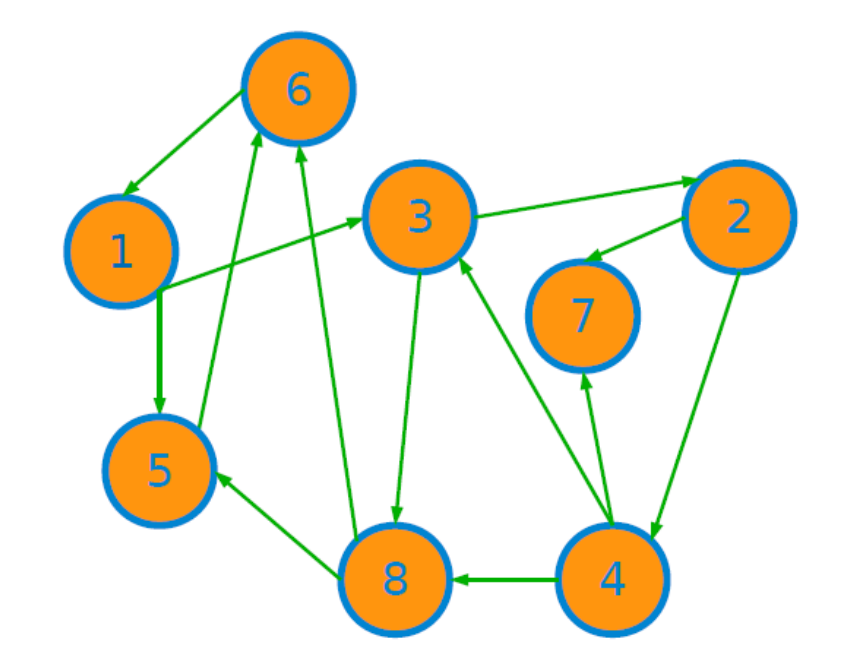
\includegraphics[scale=0.5]{figures/graph_ex.png}
\caption{This is an example graph to demonstrate how different memory accesses would occur during a breadth-first search algorithm.  The arrows in figure 2 denote the order that would normally be followed by employing a vertex-centric approach to graph processing.  }
\end{figure}

% Figure 2
\begin{figure}
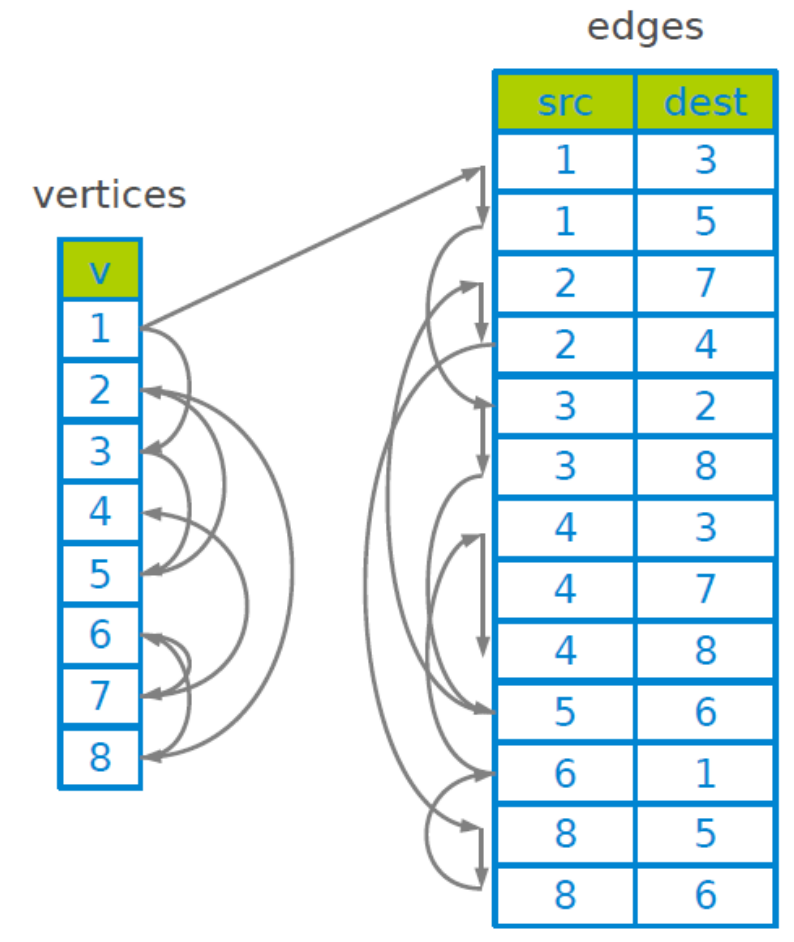
\includegraphics[scale=0.45]{figures/nodes_order.png}
\caption{The two tables represent both the vertex and edge access patterns for the graph in figure B when performing a breadth-first search.  The order of these accesses are the case for most vertex-centric models.  X-streams proposed edge-centric graph library would make the memory accesses to the edge data sequential.  The benefit of this reordered access pattern is improved data locality and bandwidth.  }
\end{figure}

\subsection{Numa-Aware Graph Structures with Polymer}

Researchers at the Shanghai Key Laboratory and the Shanghai Jiao Tong University have presented a detailed study of NUMA characteristics and their impact on the efficiency of graph-analytics.  NUMA refers to non-uniform memory access, which is a computer memory design used in multi-processing, where the memory access time depends on the memory location relative to the processor.  NUMA can be beneficial because it allows processors to access their own local memory faster than memory that is local to another processor or shared between other processors.  However, at the moment, NUMA can only be used on a limited number of architectures and with a limited number of jobs.  When applied to large scale graph processing, it was found that random or interleaved allocation of graph data is bad for data locality and therefore parallelism.  Also, it was found that sequential memory accesses have a higher bandwidth than their random counter-parts.$^{[8]}$  

Zhang, et al. proposed Polymer, a NUMA-aware graph-analytics system on multi-core that can be used to convert random remote accesses into sequential remote accesses.  Polymer was influenced by X-stream, mentioned above, and Ligra, a vertex-centric graph processing model.$^{[8]}$  Polymer classifies its data into two separate categories: graph topology data, and application-defined data.  Graph topology refers to vertex and edge data that are always accessed on their own threads.  Application-defined data refers to data whose memory locations are static but the data will be updated dynamically.  An example of application-defined data would be ranks of a web page in the PageRank algorithm, since the rank changes based on the given query.  Vertex-centric approaches like Ligra iterate over all active vertices in both scatter and gather phases and the vertex data is propagated outwards.  Edge-centrix models like X-stream iterate over all edges rather than vertices to avoid random accesses to edges.  The two main reasons that graph processing models like Ligra and X-stream don't translate well to NUMA platforms are data layout and the data access strategy.$^{[8]}$  

The two general phases of graph-analytics are graph construction and graph computation.  In current models, long-term in-memory data structures like graph topology and application-defined data are allocated and initialized by multiple construction threads on different NUMA nodes.  This data is then bound to their respective nodes at the computation stage.  With most default allocation policies there ends up being a discrepancy between the allocating threads and the processing threads which results in an interleaved page allocation pattern.$^{[8]}$  This \textit{interleaving} effect causes poor data locality and therefore a compromised performance because of the large number of remote and random memory accesses.  Remote accesses suffer a noticeably higher latency than sequential accesses.  Also, sequential remote accesses have a much higher bandwidth than both random local and random remote.  When dealing with vertex-centric approaches, even when local accesses to in-memory data structures are manually arranged in sequential order the remote accesses are coupled with random orders and simultaneous remote accesses by threads from different processors can cause other complications down the line.  When working with edge-centic systems that utilize tiling strategies, each core is able to process a partition during the scatter/gather phase.$^{[8]}$  However, even in the best case when remote access is sequential, additional overhead and memory allocation is common and it can be computationally expensive to identify the state of an edge as opposed to the state of a vertex.  

The goal of Polymer was to provide a new system that would address the latency and access problems addressed above.  It uses the typical scatter/gather pattern that many graph libraries follow.  Polymer assumes that the graph topology is immutable during graph computation.  One of the most influential results from the Polymer model is its use of NUMA-aware graph partitioning.  Because the Polymer system views NUMA machines as distributed systems, it relies on partitioning its graph data structures across all nodes in the system.$^{[8]}$  This is similar to models like Pregel and Gunrock, but different from the X-stream graph processing library.  Partitioning is usually accomplished by finding all edges with a source vertex to a single node, but this has the side-effect of added random remote access for application-defined data.  Therefore, Polymer accomplishes this by only gathering edges that are connected to a target vertex in a NUMA node.  

By using Polymer as an influence, and borrowing techniques for how to deal with non-uniform memory access aware graph analytics, we can borrow techniques that will help achieve a better performance when invoking SIMD instructions on graph data.  

\subsection{Handling Indirect Memory References}

Researchers at MIT have presented a library called \textbf{milk} that acts as a C/C++ language extension that allows programmers to annotate memory bound loops concisely.$^{[9]}$  It relies on a number of optimized intermediate data structures to transform random indirect memory references into batches of efficient sequential DRAM accesses.  Ideally some of the same ideas from Kiriansky, Zhang, and Amarasinghe can be applied to the problem of adding SIMD instructions to large-scale graph processing.  Indirect memory references in code appears something like this:
\begin{verbatim}
for (int i = 0; i < N; i++)
    count[d[i]]++;
\end{verbatim}
Because the index of the count array is dependent on the value stored for that iteration's d[i], the compiler is unable to predict its value at compile-time.  This causes complications when attempting to vectorize such code due to possible dependencies.  Many common graph algorithms display similar code structure.  This is because there's often a nested loop where the outer loop is iterating over all vertices in the graph, while an inner loop iterations over all edges coming off of the highlighted vertex for that iteration.  Due to this nested loop structure, the order that the algorithm operates on the vertices/edges in the graph is not always necessarily known at compile time, and therefore relies on dynamic memory accesses and allocation (see figure 2).  

Additionally, most real-world graphs and data sets have working sets that exceed the cache capacity and often experience bottlenecking by the DRAM, whose bandwidth, historically, has been known to increase at a much slower rate than the CPU and the latencies have barely improved.$^{[9]}$  These are the problems that the creators of milk are attempting to amortize.  The first thing they note is that random memory accesses are generally $10$ to $20$ times slower than sequential memory accesses.  This is due to the fact that memory hierarchy is optimized for sequential accesses for DRAM all the way to the cache level.  Sequential accesses are better because they benefit from the spatial locality of the DRAM chip rows.  Depending on the specific architecture, when DRAM is read from/written to, and entire DRAM row is loaded into a buffer of generally $8$ to $16$KB.$^{[9]}$  Therefore, if there are a lot of read/writes to locations in the same DRAM row, speedups will be greatly improved as they don't incur the costly latencies of loading a new row on each iteration.  However, random accesses don't experience this benefit and suffer a much high page fault rate.  Currently, the technology exists to use certain schedulers to reorder requests in a way that will minimize the number of page faults.  This is promising, but these controllers only have a limited window of future requests they can view, generally 48 cache lines per memory channel.  This type of out-of-order execution allows for multiple long delay memory accesses to be handled based on the limited hardware structure.$^{[9]}$  At the moment, each core on a CPU can handle around $10$ demand requests given that all requests fit within the window of future requests.  The greatest limitation to memory level parallelism is the capacity limits for resources requested in first-in first-out order.  In this way, if you have a loop with a large number of instructions per memory load you may experience reduced levels of parallelism.  Some other factors that can reduce instruction level parallelism are increased branch mispredictions and added atomic operations that can drain reorder buffers.  What milk offers is the ability to effectively expand the window of future operations to handle possibly billions of random accesses.$^{[9]}$  

Most of the performance improvements from invoking milk instructions come from reordering the memory accesses to take better advantage of cache spatial and temporal locality.  This is done by partitioning all indirect references to the same memory location within the cache capacity.  If done poorly, the act of reordering these memory references has the potential to actually the hurt the data locality even worse and output an even worse performance than the original due to increased overhead.  Therefore, milk places emphasis on keeping any additional bandwidth low by only using the efficient sequential DRAM references.  While data transformations require overhead in the form of added clock cycles and sequential DRAM bandwidth, these overheads are kept to a minimum.$^{[9]}$  The execution model of the milk library is similar to the reduce stage in MapReduce.  Performance improvements are first achieved by grouping references into cache-sized partitions.  Next, indirect memory reference expressions are evaluated as tags, where tags can be combined with other tags.  These variables are able to be initialized with any dynamically evaluated expression and are also written into temporary buffer data structures.  Tags are then partitioned into clusters in a way so that the maximum cache line and DRAM page locality is achieved for access.  Sometimes its the case that when too many partitions are required then this step is repeated multiple times.  The final step is when a specific part of the program is executed using a dynamically constructed context which is valid for each thread.  These steps are all part of the \textit{collection}, \textit{distribution}, and \textit{delivery} phases of the milk programming model.$^{[9]}$  

By employing this model to handle some of the problems mentioned above, programmers are able to easily modify code to better handle indirect memory references with milk.  The authors' final results show that when compared to traditional graph processing techniques being run across a suite of popular graph applications, milk was able to deliver performance gains of up to three times.  The same ideas presented in milk, especially those concerning nested array structures, directly impact the work of adding streaming SIMD extensions to common graph algorithms like PageRank, betweenness centrality, etc.  

\section{Limitations}

So far we have looked at three proposed solutions for handling large graphs and associated algorithms.  Both Pregel and Gunrock are programming models created to make it simple for developers to incorporate their APIs into their existing code with minimal effort and deliver better performance.  The third method takes a less industry driven approach to create an optimized methodology for irregular applications, which include many graph based algorithms.  However, none of these proposed solutions are perfect.  For one, Google's Pregel is not yet an open source project and it remains difficult to implement without the resources at Google's disposal.  Gunrock is open source and has a lot of associated documentation about how it operates.  However, it was specially designed for use by only GPUs and therefore cannot easily be ported to work universally on CPUs.  

There are a number of areas that all of these projects haven't fully explored.  For example, Gunrock's betweenness centrality did not take task parallelism into account.  Also, while Pregel already works well with graphs contains billions of nodes, there's always the need for improvement.  Perhaps by relaxing the synchronicity of the model to avoid the cost of faster workers having to wait frequently between supersteps, this technique could be scaled to handle even larger graphs.  Also, all of these projects target sparse graphs/matrices.  While most of the graphs that exist in practice are sparse, further research could be done to find ways to efficiently process large dense graphs.  Future SIMD work includes being able to apply the existing methodology to other classes of irregular applications like adaptive methods and pointer traversal applications.  For this to happen, tile sizes and other variables would need to be experimented with.  

As discussed earlier, some of the most common graph algorithms are things like shortest path algorithms, betweeness centrality, and traversal methods like breadth first search.  When implemented, these are often abstracted to operate on adjacency matrices, which become more and more sparse as the number of nodes in the graph increases.  An algorithm like breadth first search has a time complexity of $O(|V| + |E|)$, where $|V|$ is the number of vertices and $|E|$ is the number of edges, since every vertex and every edge will be explored in the worst case.  Of course the number of edges may vary depending on how sparse the graph and corresponding matrix are.  However, graphs representing social networks or websites can have an extremely high number of vertices, let alone edges, so optimizing these kinds of algorithms is desired.  Another common application for graphs are shortest path problems.  There are a number of such techniques and solutions, but perhaps the most famous is Dijkstra's algorithm for finding the single source shortest path between a source node and every other node in the graph.  Dijkstra's algorithm has a worst case performance of $O(|E| + |V|\log|V|)$, so again this increases as the size of the graph increases.  Finally, betweenness centrality is commonly used as a metric for determining a given node's centrality in a network.  The betweenness centrality of a node is equal to the number of shortest paths from all vertices to all others that pass through that node.  Clearly this builds off shortest path applications like Dijkstra's algorithm since you have to sum the number of all shortest paths to get the BC value.  

Common graph applications like breadth first search (BFS), single source shortest path (SSSP), betweenness centrality (BC), PageRank, etc. are all iterative algorithms and therefore should be, at least at some level, vectorizable.  The goal of this project is to determine whether streaming SIMD extensions (SSE) can be applied to these algorithms in a similar way to existing models like Google's Pregel and Gunrock to improve their performance on large scale graphs.  The challenge to doing this will be to determine where parallelism can be extracted from the inner loops based on loop dependencies.  It is essential that any SIMD solution to this problem carefully evaluate read-after-write dependencies in order to maximize both the inter and intra-iteration parallelism from the process.  By representing the vertices and edges of the graph in an adjacency matrix instead of abstracting these objects into classes, we are able to store the values in SIMD vectors and operate on them at a data level of parallelism.  

\section{Methodology \& Results}

To evaluate the effect of applying SIMD extensions to large graph processing, the GraphBIG benchmark was used.  GraphBIG is a graph benchmarking effort initiated by Georgia Tech HPArch and inspired by IBM System G.  It supports a wide selection of workloads from both the CPU and GPU side and it covers a broad spectrum of graph computing and fulfills multiple major requirements including framework, representativeness, coverage, and graph data support.  GraphBIG includes code for many benchmarks including breadth first search, depth first search, PageRank, etc.  The four I focused on were PageRank, betweenness centrality, triangle count, and Gibbs inference.  The latter two are less common but I selected them because they had the most dense kernel code on which I could apply vector instructions.  A common pattern seemed to be algorithms where there were little to no binary operations like addition or subtraction; instead there were just repeated loops where elements were pushed to and popped from queues and other custom data structures.  GraphBIG also seemed to have a high percentage of benchmarks with these binary operations than other benchmarks I investigated, like the Rodinia benchmark.  All of the benchmarks used for this project were tested on a graph that was composed of 10000 vertices and 29790 edges.  The triangle count algorithm is pretty straight-forward.  The number of triangles in a graph is a computationally expensive graph statistic which is frequently used in complex network analysis, in various random graph models, and in important real world applications such as spam detection, uncovering hidden structures in the Web and link recommendation.  Gibbs inference, or Gibbs sampling, is a Markov chain Monte Carlo algorithm for obtaining a sequence of observations which are approximated from a specified multivariate probability distribution, when direct sampling is difficult.  The sequence can be used to approximate the joint distribution, to approximate the marginal distribution of one of the variables or some subset of them, or to compute an integral, such as the expected value of one of the variables.  Typically, some of the variables correspond to observations whose values are known and hence do not need to be sampled.  

Streaming SIMD extensions (SSE2 through SSE4) were added into the code for the benchmarks described above.  SSE is a SIMD instruction set extension to the x86 architecture, designed by Intel and introduced in 1999 in their Pentium III series processors.  SSE contains 70 new instructions, most of which work on single precision floating point data.  SIMD instructions can greatly increase performance when the same operations are to be performed on multiple data objects.  Generally, these applications tend to be related to fields such as digital signal processing and graphics processing.  The first SIMD instruction set proposed by Intel was MMX, which was problematic in that it reused existing floating point registers making the CPU unable to work on both floating point and SIMD data at the same time.  SSE improved upon the old model as it operates a new independent register set and adds sever integer instructions that work on MMX registers.  GraphBIG is written in C++ and the code is compiled via GCC with the \textbf{-03} flag.  In the first round of testing, vectors with a 128 bit width were used.  These are sufficient for storing 4 32-bit integer or single precision floating point values, 2 64-bit double precision floating point values, or 8 16-bit short integer values.  In the vectorized PageRank implementation, three single-precision floating point vectors were instantiated along with another vector of all zero values.  Before SIMD instructions can be applied to these vectors they need to be aligned along 16 byte boundaries and adequate memory allocated for each.  If unaligned, or aligned incorrectly, the given operations may not behave as intended or the code simply may not compile.  These SSE vectors and their respective operations were applied to the main for loop of the PageRank kernel.  The first operation was a subtraction between the current pointer's value and the old pointer's value.  This result was then squared and loaded into an array.  This sort of computational pattern is a prime candidate for vectorization due to it's dense kernel and few dependencies.  However, the first line of the for loop was a function call to find the next vertex to operate on.  The order that this function returned vertices was not linear and therefore difficult to vectorize directly.  Instead, the loop was unrolled (by a factor of $4$), and four new variables were instantiated.  From these, subsequent vector instructions could be performed easily.  Initially a \textbf{\_mm\_load\_ps()} function call was made to load aligned array elements into SSE vectors.  Then the subsequent subtraction and multiplication operations were executed in parallel on the vectors.  The main result of this loop was a reduction on the elements in the array into a single sum, so on each iteration two horizontal adds were performed with the \textbf{\_mm\_hadd\_ps()} function call, and finally the result is stored back into the original sum variable.  After applying SIMD instructions to GraphBIG's PageRank algorithm, a speedup of $1.17$ was obtained.  While this is not a huge performance improvement, it is probably sufficient to show that there exists the potential for improvements to large-scale graph processing via vectorization.  However, it should be noted that some portion of this speedup may be attributed to the loop-unrolling alone, which can provide greater data locality, resulting in increased performance.  The results from the four benchmarks are displayed in Figure 3.  

% Figure 3
\begin{figure}
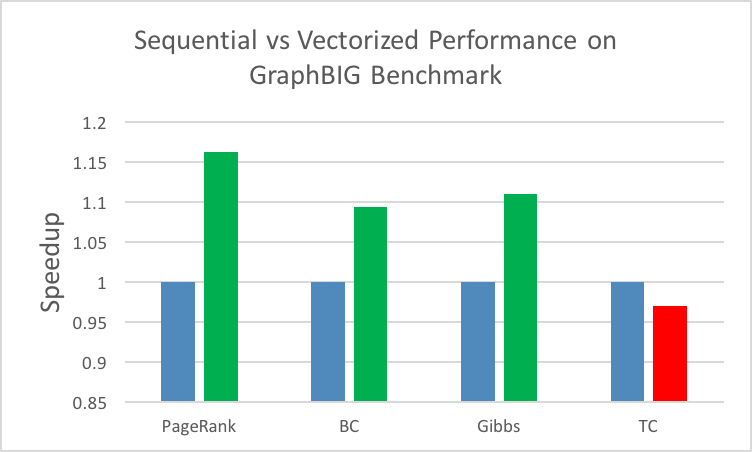
\includegraphics[scale=0.7]{figures/benchmark1.png}
\caption{As shown in the graph, PageRank, betweenness centrality, and the Gibbs inference benchmarks all displayed relatively small amounts of speedup.  In the case of the triangle count benchmark, the overhead of packing and unpacking vector registers actually hurt the overall performance.  }
\end{figure}

Adding SIMD instructions to the betweenness centrality program displayed similar speedups.  The main difference between this benchmark and PageRank was the use of short integers in the vectors.  In this case, 8 16-bit short integer values could be packed into a single vector at once.  Similar loop-unrolling was performed as a way to handle custom data structures without arithmetic instructions.  This benchmark also contained several branch statements in the form of the $?$ format.  These were vectorized by using a mask vector to correctly operate on the necessary vector elements.  Of the four benchmarks tested, the triangle count benchmark was the only one that actually performed worse than the sequential version.  Upon examination, many of the loops in the triangle count benchmark were short, in the sense that they rarely repeated more than $4$ times, making vectorization useless and causing the added overhead of packing/unpacking vectors to hurt the performance.  There were a number of challenges to the vectorization of graph algorithms.  The first was that sometimes there was simply no dense kernel of arithmetic instructions to vectorize, but instead appending and popping to/from queues and other custom objects.  For vectorization to be possible in these cases one would need to change the entire structure of the code so that the use of SIMD instructions would be possible.  Another challenge is dependencies.  Because a lot of common graph algorithms perform updates on outgoing edges, the order of traversal can be important and simultaneous writes can cause race conditions.  Additionally, some benchmarks do not have enough iterations of the inner loop to use vectorization.  In these cases, the overhead of added intrinsics often makes the performance worse than the sequential code.  In these cases, it may be possible to employ the use of superword level parallelism to extract as much parallelism as possible from these loops.  Finally, some benchmarks displayed a divergence of the number of outgoing edges for each vertex.  If there is a large disparity, this is often challenging for parallelism.  In an ideal case all nodes would have a large number of edges.  However, we know that this is not often the case.  Especially as graphs grow in size, they generally become more sparse.  There are essentially two ways to handle this problem: either change the problem to focus only on dense graphs, or change the input to be more dense.  

Additionally, the PageRank benchmark was also performed using the longer vector widths from AVX-512.  AVX-512 are 512-bit extensions to the 256-bit Advanced Vector Extensions SIMD instructions for x86 instruction set architecture proposed by Intel in 2013.  It is supported by Intel's Xeon Phi x200 Knights Landing processor.  It consists of multiple extensions not all meant to be supported by all processors implementing them.  Only the core extension AVX-512F is required by all implementations.  By providing a vector of width 512-bits, the programmer is able to perform simultaneous operations on 16 32-bit integers or 32-bit single precision floating point values.  This is 4 times the amount that previous SSE vector registers could handle.  The general syntax and semantics of AVX-512 over earlier SSE intrinsics is similar.  After applying these wider vector registers to the PageRank algorithm, a speedup of nearly 2 times was reported.  It's unsurprising that an increased level of data level parallelism yields a better performance.  The results from the addition of the AVX-512 vectors are shown in figure 4.  

% Figure 4
\begin{figure}
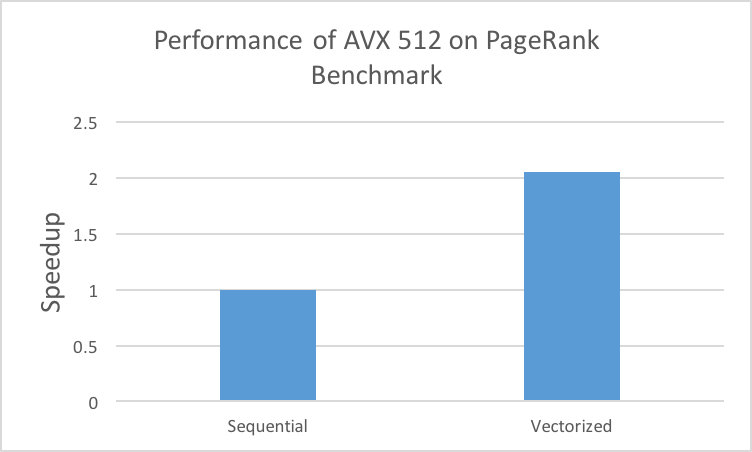
\includegraphics[scale=0.7]{figures/benchmark_avx.png}
\caption{By using vector registers of length 512 bits on the PageRank benchmark, and performance speedup of roughly $2 \times$ was reported.  }
\end{figure}

\section{Conclusion}

In conclusion, graph processing is a common way to model a number of relationships, from websites on the internet to people on social networks.  As big data becomes more and more of a reality this causes problems when attempting to process very large graphs efficiently.  Fortunately, a lot of existing research has been done to find ways to handle these large graphs.  The Pregel model by Google and Gunrock are two programming models that can be used to extract more parallelism from existing graph techniques.  Other memory management solutions from the X-stream model and the milk language extension can be applied to this problem.  Four different graph algorithms from the GraphBIG benchmark were vectorized, at least partly, using streaming SIMD extensions.  From the results, a mild speedup was noticed using 128-bit wide vector registers but the 512-bit registers provided a much more noticeable performance improvement.  Through this preliminary analysis of large-scale graph processing, we can conclude that applying SIMD instructions to graph algorithms is possible to achieve improved runtimes.  
%\\
%\\
%\\

\section{Final notes}
The code for the benchmark algorithms with added SIMD capability can be found at \url{https://github.com/alexanderjpowell/cs_680_research_project}.  The following instructions explain how to compiler and run, after the source has been cloned from the above listed repository.  Note: Apart from the AVX-512 implementation of PageRank, these were tested on the department BGs.  


\begin{itemize}
\item \# For the four benchmarks described in the results, 
\item \# navigate to the benchmark directory of graphBIG
\item $>$ cd cs\_680\_research\_project/graphBIG/benchmark/
\item $>$ make clean all \# compile the code
\item $>$ cd bench\_pageRank \# or bench\_betweennessCentr, 
\item \# bench\_gibbsInference, and bench\_triangleCount
\item $>$ make run
\item $>$ cat output.log \# To view results
\end{itemize}

\# For KNL-machine:
\begin{itemize}
\item $>$ cd cs\_680\_research\_project/graphBIG\_avx/benchmark/
\item $>$ make clean all
\item $>$ cd bench\_pageRank
\item $>$ make run
\item $>$ cat output.log
\end{itemize}


This is also explained in the README.  All necessary flags and libraries have been added to the Makefiles.  

As far as timing, most research and coding for PageRank and betweenness centrality were finished before the last day of classes.  After November $30^{\text{th}}$, additional work was done to modify the code for Gibb's inference and triangle count algorithms, although these results were not as promising as the first two.  Some modifications were also made to the AVX-512 version of PageRank to fix an alignment issue.  The majority of the report was also written after November $30^{\text{th}}$.  


% no \IEEEPARstart
%This demo file is intended to serve as a ``starter file''
%for IEEE conference papers produced under \LaTeX\ using
%IEEEtran.cls version 1.8b and later.
% You must have at least 2 lines in the paragraph with the drop letter
% (should never be an issue)
%I wish you the best of success.
%\hfill mds
%\hfill August 26, 2015

%\subsection{Subsection Heading Here}
%Subsection text here.


%\subsubsection{Subsubsection Heading Here}
%Subsubsection text here.


% An example of a floating figure using the graphicx package.
% Note that \label must occur AFTER (or within) \caption.
% For figures, \caption should occur after the \includegraphics.
% Note that IEEEtran v1.7 and later has special internal code that
% is designed to preserve the operation of \label within \caption
% even when the captionsoff option is in effect. However, because
% of issues like this, it may be the safest practice to put all your
% \label just after \caption rather than within \caption{}.
%
% Reminder: the "draftcls" or "draftclsnofoot", not "draft", class
% option should be used if it is desired that the figures are to be
% displayed while in draft mode.
%
%\begin{figure}[!t]
%\centering
%\includegraphics[width=2.5in]{myfigure}
% where an .eps filename suffix will be assumed under latex, 
% and a .pdf suffix will be assumed for pdflatex; or what has been declared
% via \DeclareGraphicsExtensions.
%\caption{Simulation results for the network.}
%\label{fig_sim}
%\end{figure}

% Note that the IEEE typically puts floats only at the top, even when this
% results in a large percentage of a column being occupied by floats.


% An example of a double column floating figure using two subfigures.
% (The subfig.sty package must be loaded for this to work.)
% The subfigure \label commands are set within each subfloat command,
% and the \label for the overall figure must come after \caption.
% \hfil is used as a separator to get equal spacing.
% Watch out that the combined width of all the subfigures on a 
% line do not exceed the text width or a line break will occur.
%
%\begin{figure*}[!t]
%\centering
%\subfloat[Case I]{\includegraphics[width=2.5in]{box}%
%\label{fig_first_case}}
%\hfil
%\subfloat[Case II]{\includegraphics[width=2.5in]{box}%
%\label{fig_second_case}}
%\caption{Simulation results for the network.}
%\label{fig_sim}
%\end{figure*}
%
% Note that often IEEE papers with subfigures do not employ subfigure
% captions (using the optional argument to \subfloat[]), but instead will
% reference/describe all of them (a), (b), etc., within the main caption.
% Be aware that for subfig.sty to generate the (a), (b), etc., subfigure
% labels, the optional argument to \subfloat must be present. If a
% subcaption is not desired, just leave its contents blank,
% e.g., \subfloat[].


% An example of a floating table. Note that, for IEEE style tables, the
% \caption command should come BEFORE the table and, given that table
% captions serve much like titles, are usually capitalized except for words
% such as a, an, and, as, at, but, by, for, in, nor, of, on, or, the, to
% and up, which are usually not capitalized unless they are the first or
% last word of the caption. Table text will default to \footnotesize as
% the IEEE normally uses this smaller font for tables.
% The \label must come after \caption as always.
%
%\begin{table}[!t]
%% increase table row spacing, adjust to taste
%\renewcommand{\arraystretch}{1.3}
% if using array.sty, it might be a good idea to tweak the value of
% \extrarowheight as needed to properly center the text within the cells
%\caption{An Example of a Table}
%\label{table_example}
%\centering
%% Some packages, such as MDW tools, offer better commands for making tables
%% than the plain LaTeX2e tabular which is used here.
%\begin{tabular}{|c||c|}
%\hline
%One & Two\\
%\hline
%Three & Four\\
%\hline
%\end{tabular}
%\end{table}


% Note that the IEEE does not put floats in the very first column
% - or typically anywhere on the first page for that matter. Also,
% in-text middle ("here") positioning is typically not used, but it
% is allowed and encouraged for Computer Society conferences (but
% not Computer Society journals). Most IEEE journals/conferences use
% top floats exclusively. 
% Note that, LaTeX2e, unlike IEEE journals/conferences, places
% footnotes above bottom floats. This can be corrected via the
% \fnbelowfloat command of the stfloats package.




% conference papers do not normally have an appendix


% use section* for acknowledgment
%\section*{Acknowledgment}


%The authors would like to thank...





% trigger a \newpage just before the given reference
% number - used to balance the columns on the last page
% adjust value as needed - may need to be readjusted if
% the document is modified later
%\IEEEtriggeratref{8}
% The "triggered" command can be changed if desired:
%\IEEEtriggercmd{\enlargethispage{-5in}}

% references section

% can use a bibliography generated by BibTeX as a .bbl file
% BibTeX documentation can be easily obtained at:
% http://mirror.ctan.org/biblio/bibtex/contrib/doc/
% The IEEEtran BibTeX style support page is at:
% http://www.michaelshell.org/tex/ieeetran/bibtex/
%\bibliographystyle{IEEEtran}
% argument is your BibTeX string definitions and bibliography database(s)
%\bibliography{IEEEabrv,../bib/paper}
%
% <OR> manually copy in the resultant .bbl file
% set second argument of \begin to the number of references
% (used to reserve space for the reference number labels box)

\newpage 

\begin{thebibliography}{1}

\bibitem{IEEEhowto:kopka}
Malewicz, Austern, Bik, Dehnert, Horn, Leiser, and Czajkowski, \emph{Pregel: A System for Large-Scale Graph Processing},\hskip 1em plus
  0.5em minus 0.4em\relax Indianapolis, Indiana: SIGMOD, 2010.
\\
\bibitem{IEEEhowto:kopka}
Wang, Davidson, Pan Wu, Riffel, and Owens, \emph{Gunrock: A High-Performance Graph Processing Library on the GPU},\hskip 1em plus
  0.5em minus 0.4em\relax University of California, Davis: PPoPP, 2016.
\\
\bibitem{IEEEhowto:kopka}
L. Chen, P. Jiang, and G. Agrawal, \emph{Exploiting Recent SIMD Architectural Advances for Irregular Applications},\hskip 1em plus
  0.5em minus 0.4em\relax The Ohio State University, Columbus, OH: CGO, 2016.
\\
\bibitem{IEEEhowto:kopka}
Dave Ankur, \emph{What are the main concepts behind Google's Pregel?},\hskip 1em plus
  0.5em minus 0.4em\relax Google, 2012.
\\
\bibitem{IEEEhowto:kopka}
L. Chen, G. Agrawal, and B. Ren, \emph{Efficient and Simplified Parallel Graph Processing over CPU and MIC},\hskip 1em plus
  0.5em minus 0.4em\relax Columbus, Ohio: IPDPS15, 2015.
\\
\bibitem{IEEEhowto:kopka}
Sreepathi Pai and Keshav Pingali, \emph{A Compiler for Throughput Optimization of Graph Algorithms on GPUs},\hskip 1em plus
  0.5em minus 0.4em\relax Austin, Texas: OOPSLA, 2016.
\\
\bibitem{IEEEhowto:kopka}
Roy, Mihailovic, Zwaenepoel, \emph{X-Stream: Edge-centric Graph Processing using Streaming Partitions},\hskip 1em plus
  0.5em minus 0.4em\relax Farminton, PA: SOSP, 2013.
\\
\bibitem{IEEEhowto:kopka}
Zhang, Chen, Chen, \emph{NUMA-Aware Graph-Structured Analytics},\hskip 1em plus
  0.5em minus 0.4em\relax San Francisco, CA, USA: PPoPP, 2015.
\\
\bibitem{IEEEhowto:kopka}
Kiriansky, Zhang, Amarasinghe, \emph{Optimizing Indirect Memory References with milk},\hskip 1em plus
  0.5em minus 0.4em\relax Haifa, Israel, PACT, September 2016.

\end{thebibliography}




% that's all folks
\end{document}




































